Consider the heterogeneous wave equation with 
\begin{align*}
\rho(x)\pd{u}{t}{2} - \pd{u}{x}{2} &= f(x,t)\\
u(x,0) &= \psi(x)\\
\pd{u}{t}{}(x,0) &= 0\\
u(0,t) &= 0\\
\pd{u}{x}{}(1,t) &= 0
\end{align*}
\begin{enumerate}
In seismic imaging problems (i.e. sonar, radar, finding oil, etc), the wave equation can be used to simulate a sound wave propagating in the $x$ direction through a medium.  Here, we assume $\rho(x)$ is the density of the medium, and that it only changes in the direction of propagation.  

\item Formulate a weak form for the above equation.  
\item Let $f= 0$ and $\rho(x) = 1$, which reduces to the standard wave equation with $c=1$.  For a pulse initial condition 
\[
\psi(x) = xe^{-100x^2}
\]
compute the finite element solution (using the matrix exponential) with $N = 63$ and $dt = .015$.  Create a 3D plot of the solution by using \verb+surf+ to plot the solution at equally spaced times from 0 to the final time $T = 2$.  Note: If you compute your solution at points $x_j$ and times $t_i$,
\[
x_j = 0, h, \ldots, 1-h, 1, \qquad t_i = 0, dt, \ldots, 2
\]
and form a matrix
\[
U_{ij} = u(x_j,t_i)
\]
then you may use \verb+surf(X,T,U)+ to compute a 3D plot of the solution, where \verb+X+ and \verb+T+ are vectors of the points $x_i$ and times $t_j$.  You may also wish to use the command \verb+shading interp+ to remove mesh lines from the 3D solution plot.  

\item Let $\rho(x)$ now be a discontinuous function
\[
\rho(x) = \begin{cases}
k_1, & x < .5\\
k_2, & x \geq .5.
\end{cases}
\]
For $N$ odd, give a formula depending on $j$ and/or $x_j$ for the entries of the mass matrix.  
\item Take $k_1 = .25$ and $k_2 = 1$.  Compute the finite element solution using the same initial condition and $N, dt$ as in (b).  What effect does the discontinuity have on the behavior of the solution over $x$ and $t$?  
\end{enumerate}

%%%%%%%%%%%%%%%%%%%%%%%%%%%%%%%%%%%%%%%%%%%%%%%%%%%%%%%%%%%%%%%%%%%%%%%%%%%%%%%%
\ifthenelse{\boolean{showsols}}{
\begin{solution}

\begin{enumerate}
\item Multiplying the equation and integrating the spatial derivative by parts gives
\[
\int_0^1\rho(x)\pd{u}{t}{2} v(x)dx + \int_0^1 \pd{u}{x}{}\pd{v}{x}{} - \left[ \pd{u}{x}{}v\right]_0^1.
\]
The boundary term vanishes after taking into account the boundary condition on $\pd{u}{x}{}(1,t)= 0$, and the condition on $v(x)$ that $v(0) = 0$.  
\item The solution for $k_1 = k_2 = 1$ is given as follows
\begin{figure}
\centering
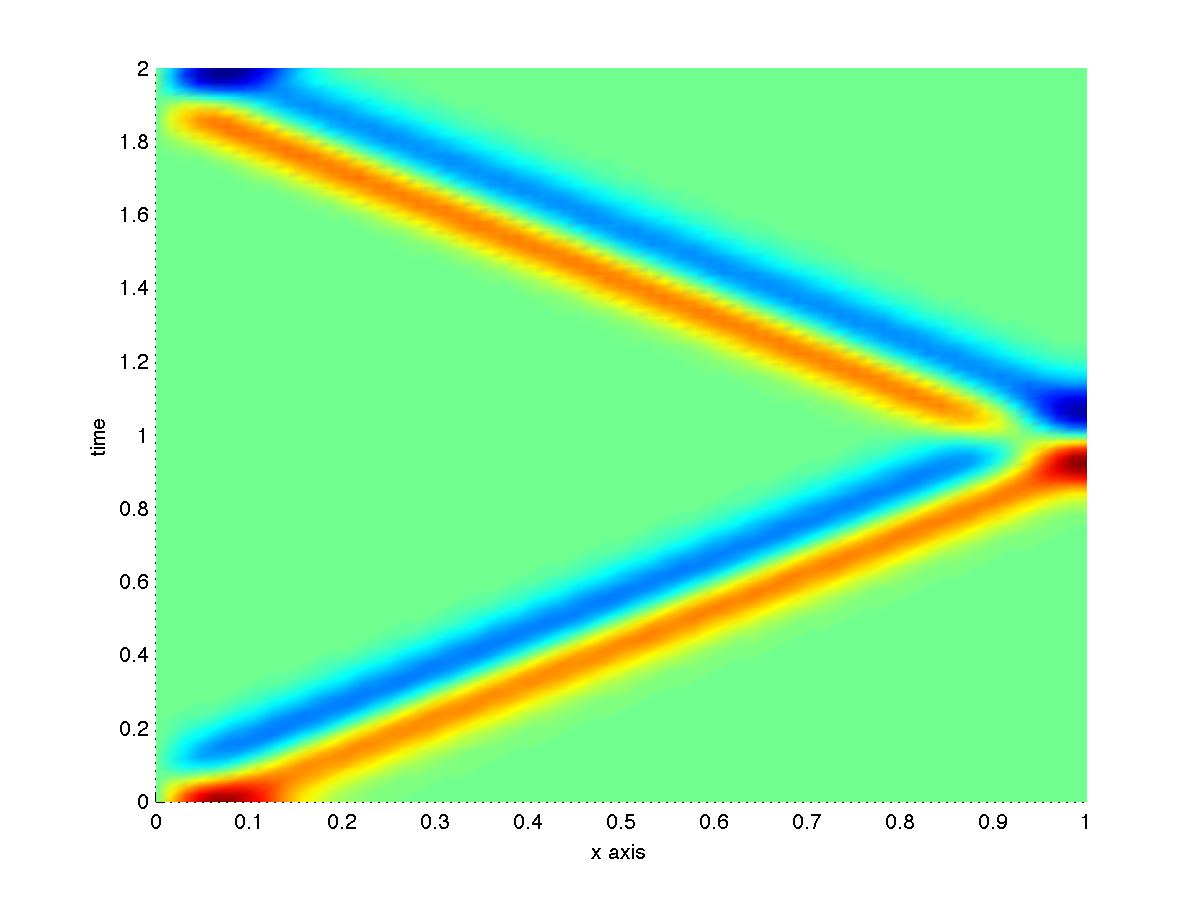
\includegraphics[width=.7\textwidth]{wavefem_1.png}
\caption{Top-down view of the solution for $k_1 = k_2 = 1$}
\end{figure}
\item If $N$ is odd, then there lies exactly one point $x_m$ such that $x_m = .5$.  Then, the mass matrix will have modified terms
\[
M_{i,i} = \begin{cases}
k_1\frac{4h}{6}, & i< m\\
(k_1 + k_2)\frac{h}{3}, & i = m\\
k_2\frac{4h}{6}, & i > m
\end{cases}, \qquad 
M_{i,i-1} = \begin{cases}
k_1\frac{h}{6}, & i\leq m\\
k_2\frac{h}{6}, & i > m
\end{cases},
\]
and $M_{i-1,i}$ can be found using symmetry of $M$.  
\item The solution shows a unique physical feature: plotting the solution over time shows that a wave propagates up to the discontinuity in $\rho(x)$, then produces two waves --- one traveling forward at a faster speed, while the other reflects off of the discontinuity and propagates backwards.  

This phenomena is observed due to the face that $\rho(x)$ is representative of density --- if density is discontinuous, it is as if there are two types of media that a wave is propagating through.  For example, if you propagate a wave through water and the wave hits rock, the wave may propagate through the rock, but it will also reflect back into the water.  

\begin{figure}
\centering
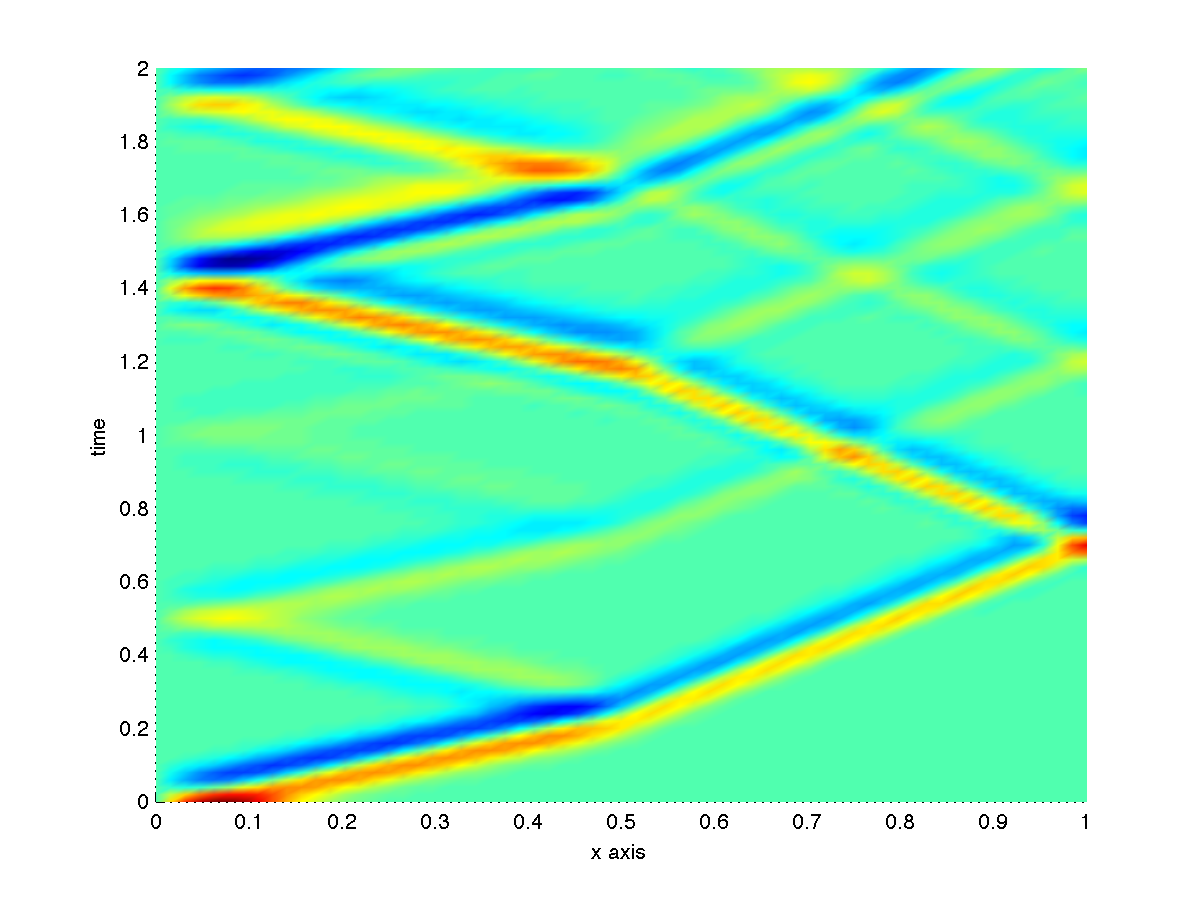
\includegraphics[width=.7\textwidth]{wavefem_2.png}
\caption{Top-down view of the solution for $k_1 = .25, k_2 = 1$}
\end{figure}

\end{enumerate}

The code that produced these plots follows.

\input wavefem_code

\end{solution}

}{}
